\documentclass[compress,xcolor=table]{beamer}

\usepackage{lmodern}

\mode<presentation>
{
	\usetheme{Madrid}      % or try Darmstadt, Madrid, Warsaw, ...
	\usecolortheme{beaver} % or try albatross, beaver, crane, ...
	\usefonttheme{serif}  % or try serif, structurebold, ...
	\setbeamertemplate{navigation symbols}{}
	\setbeamertemplate{caption}[numbered]
} 

\makeatletter
\setbeamertemplate{headline}{%
	\begin{beamercolorbox}[ht=2.25ex,dp=3.75ex]{section in head/foot}
		\insertnavigation{\paperwidth}
	\end{beamercolorbox}%
}%
\makeatother

\makeatletter
\newenvironment{withoutheadline}{
	\setbeamertemplate{headline}[default]
	\def\beamer@entrycode{\vspace*{-\headheight}}
}{}
\makeatother

\usepackage[english]{babel}
\usepackage[utf8]{inputenc}
\usepackage{xcolor}
\usepackage{listings}
\usepackage{textpos}
\newcommand\citem[1]{\item[{[#1]}] }
%\usepackage{enumitem}% http://ctan.org/pkg/enumitem

\lstset
{
	language=[LaTeX]TeX,
	breaklines=true,
	basicstyle=\tt\scriptsize,
	%commentstyle=\color{green}
	keywordstyle=\color{red},
	%stringstyle=\color{black}
	identifierstyle=\color{orange},
}

\newcommand{\backupbegin}{
	\newcounter{finalframe}
	\setcounter{finalframe}{\value{framenumber}}
}
\newcommand{\backupend}{
	\setcounter{framenumber}{\value{finalframe}}
}

\newenvironment<>{varblock}[2][.9\textwidth]{%
	\setlength{\textwidth}{#1}
	\begin{actionenv}#3%
		\def\insertblocktitle{#2}%
		\par%
		\usebeamertemplate{block begin}}
	{\par%
		\usebeamertemplate{block end}%
\end{actionenv}}

%\usepackage{outlines}
\setbeamercolor{itemize item}{fg=red,bg=white}

\usepackage{multirow}
\usepackage{caption}
\usepackage{subcaption}

%%% TITLE
\title[FG-ML5G]{Decentralized learning implications on the performance of dense WLANs}
\author[F. Wilhelmi]{
\includegraphics[width=\textwidth,height=0.13\textheight,keepaspectratio]{img/logo_upf.jpg}\\~\\Francesc Wilhelmi}
\institute[UPF]{Co-authors: B. Bellalta, C. Cano, G. Neu, A. Jonsson \& S. Barrachina-Mu\~noz}
\date[Geneva, 30/01/18]{Geneva, 30/01/18}

\AtBeginSection[]
{
	\begin{frame}<beamer>
	\frametitle{Outline}
	\tableofcontents[currentsection,currentsubsection]
\end{frame}
}

\begin{document}

\begin{withoutheadline}
	\begin{frame}
		\titlepage
	\end{frame}
\end{withoutheadline}

\begin{frame}{Table of contents} % and our simple frame
	\tableofcontents
\end{frame}

%%% INTRODUCTION
\section{Introduction}

% Problem description
\subsection{}
\begin{frame}{Problem description}
%\begin{columns}
%	\begin{column}{6cm}
		\begin{block}{Spatial Reuse (SR) enhancement in dense Wireless Networks}
			\begin{itemize}
				%\pause
				\item Transmit Power Control (TPC)
				%\pause
				\item Carrier Sense Threshold (CST) adjustment
				%\pause
				\item Dynamic Channel Selection (DCA)
			\end{itemize}
		\end{block}	
		%\end{column}
		%\pause
%	\end{column}
\begin{columns}
	\begin{column}{6cm}
		\begin{figure}
			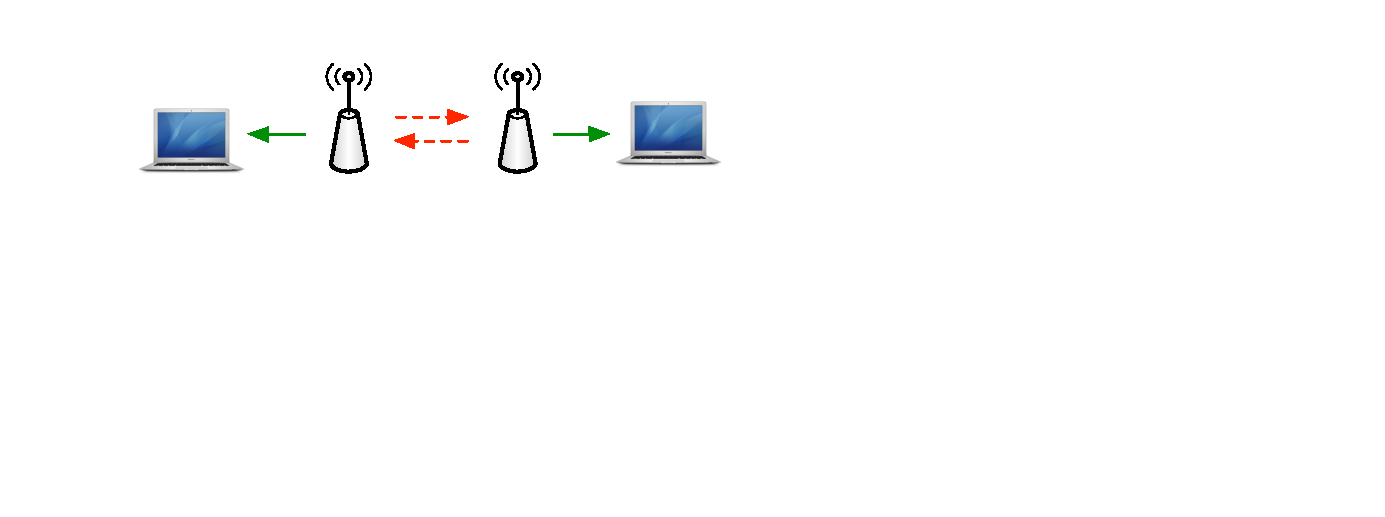
\includegraphics[width=\textwidth,height=0.15\textheight,keepaspectratio]{img/scenario_1_conf_a}
			\caption{Limited performance}
		\end{figure}
		\end{column}	
		\begin{column}{6cm}
		\begin{figure}
			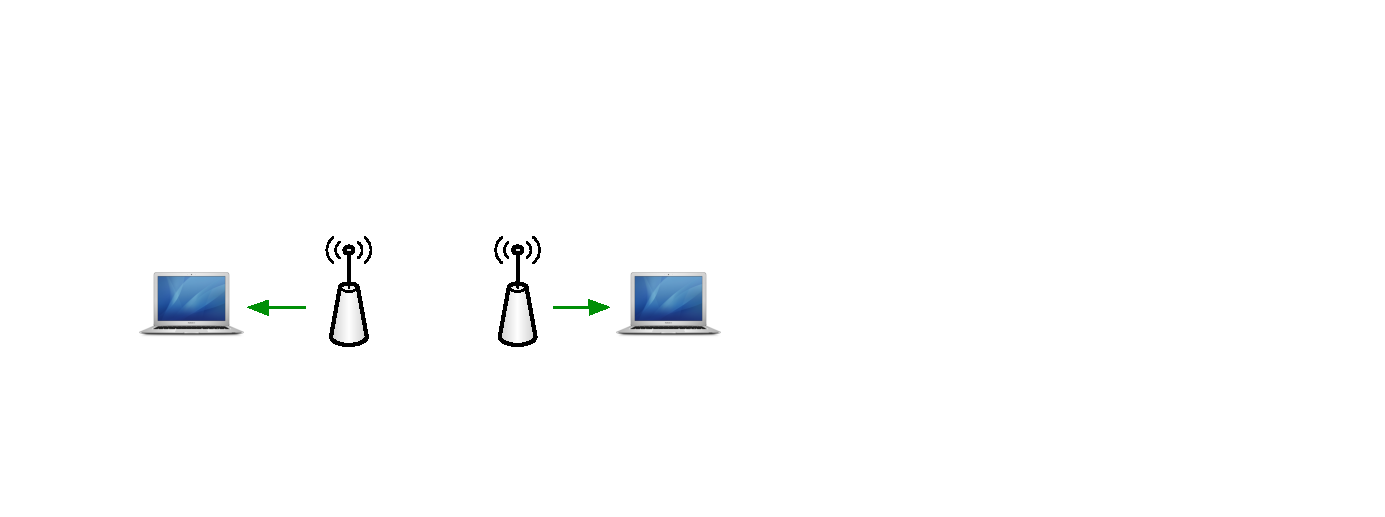
\includegraphics[width=\textwidth,height=0.15\textheight,keepaspectratio]{img/scenario_1_conf_b}
			\caption{Enhanced spatial reuse}
		\end{figure}		
	\end{column}	
	
\end{columns}

\end{frame}

% Context
\subsection{}
\begin{frame}{Context - Use case}
\begin{columns}
	\begin{column}{7cm}
		\begin{itemize}
			\item Dense IEEE 802.11 WLANs
			\begin{itemize}
				\item Unplanned (chaotic deployments)
				\item Decentralized (local information only)
			\end{itemize}
			\item Online learning through adversarial Multi-Armed Bandits (MABs)
		\end{itemize}
	\end{column}	
	\begin{column}{4.5cm}
		\begin{figure}
			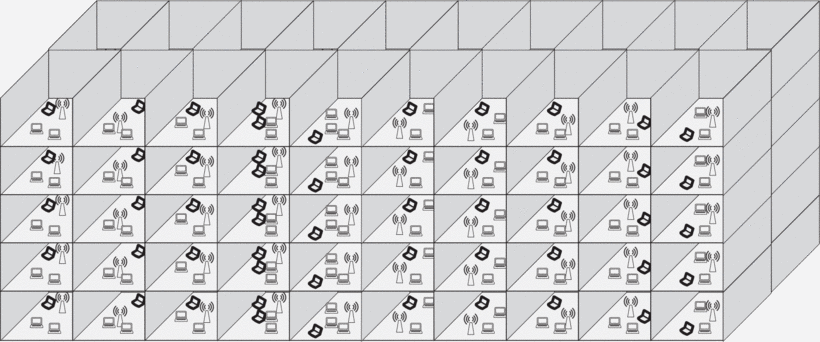
\includegraphics[width=\textwidth,height=0.4\textheight,keepaspectratio]{img/TGax_scenario}
			\caption{TGax residential scenario. Image retrieved from [1].}
		\end{figure}		
	\end{column}	
\end{columns}

\end{frame}

% ML motivation
\subsection{}
\begin{frame}{Why MABs?}
		\begin{enumerate}
			\item Uncertainty $\rightarrow$ no information exchange
			\item Adversarial setting $\rightarrow$ the reward is influenced by the environment	
			\item Complex interactions:
			\begin{table}[h!]
				\centering
				\resizebox{0.8\textwidth}{!}{\begin{tabular}{|c|c|c|c|c|}
						\hline
						\multirow{2}{*}{\begin{tabular}[c]{@{}c@{}}\\ \textbf{Action}\end{tabular}} & \multicolumn{4}{|c|}{\textbf{Effect}} \\ \cline{2-5} 
						& \begin{tabular}[c]{@{}c@{}}Parallel\\ Transmissions\end{tabular}  & Data Rate & \begin{tabular}[c]{@{}c@{}}Collisions probability\\ (by hidden node)\end{tabular} & \begin{tabular}[c]{@{}c@{}}Energy\\ Consumption\end{tabular}\\ \hline
						$\uparrow$ Power & $\downarrow$ & $\uparrow$ & $\downarrow$ & $\uparrow$ \\ \hline
						$\downarrow$ Power & $\uparrow$ & $\downarrow$ & $\uparrow$ & $\downarrow$ \\ \hline
						$\uparrow$ CCA & $\uparrow$ & - & $\uparrow$ & $\uparrow$* \\ \hline
						$\downarrow$ CCA & $\downarrow$ & - & $\downarrow$ & $\downarrow$* \\ \hline
					\end{tabular}
				}
				\caption{Effects of TPC and CST adjustment}
				\label{tbl:cca_tpc_effects}
			\end{table}				
		\end{enumerate}
		%\pause
		\begin{center}
			\begin{minipage}{15cm}			
				\begin{varblock}[9cm]{}
					\centering
					Need to find an \textbf{approximation} of the optimal solution, rather than computing it.
				\end{varblock}
			\end{minipage}
		\end{center}
\end{frame}

%%% RELATED WORK
\section{Related Work}

\begin{frame}{Related Work}
	
	\begin{block}{Surveys}
		\centering
		\begin{itemize}
			\item Self-Organized Networks (SONs) [1]
			\item Cognitive radio [2]
			\item Wireless Sensor Networks (WSN) [3, 4]
			\item Ad-hoc networks [5]
		\end{itemize}
	\end{block}
	
	\begin{block}{Related to this problem}
		\centering
		\begin{itemize}
			\item Q-learning for channel selection [6-9] and power adjustment [10, 11]
			\item MABs to Power control in D2D networks [12, 13]
			\item MABs to DCA \& TPC [14]
			\item Structured MABs for combinatorial optimization problems [15, 16]
			\item MABs for decentralized channel access [17, 18]
		\end{itemize}
	\end{block}
	
\end{frame}

%%% SYSTEM MODEL
\section{System Model}

% Scenario and System model
\subsection{}
\begin{frame}{The Multi-Armed Bandit problem}

	\begin{block}{Formal definition}
		A game in which the following steps are repeated in $t=1,2,\dots,T$:
		\begin{enumerate}
			\item The environment fixes an assignment of rewards $r_{a,t}$ for each action $a\in[K] \stackrel{\text{def}}{=} \left\{1,2,\dots,K\right\}$,
			\item the learner chooses action $a_t\in[K]$,
			\item the learner obtains and observes reward $r_{a_t,t}$
		\end{enumerate}
	\end{block}	

	\begin{figure}
		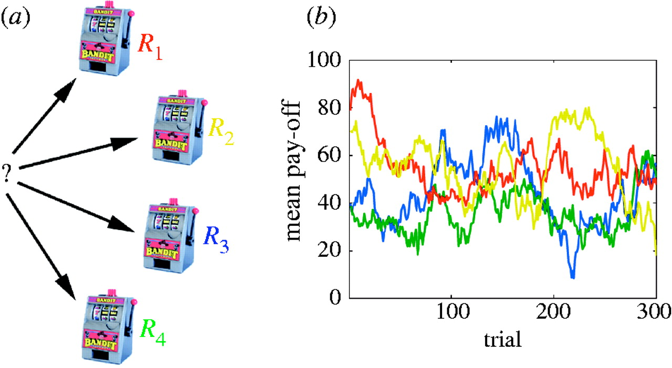
\includegraphics[width=\textwidth,height=0.4\textheight,keepaspectratio]{img/hidden_reward}
	\end{figure}

\end{frame}

% Scenario and System model
\subsection{}
\begin{frame}{MABs application into Decentralized WLANs}
	\begin{block}{Use case}
		\begin{itemize}
			\item Adversarial setting ($N$ WLANs make actions simultaneously)
			\item Actions consist in \{channel, tx. power, CCA\} combinations
			\item The reward is \textbf{selfishly} set as the own throughput
			\item Action-selection procedure: Thompson sampling [19]
		\end{itemize}
	\end{block}	
\end{frame}

%%% RESULTS
\section{Simulation Results}

% Scenario and situations
\subsection{}
\begin{frame}{Selfish learning - Scenario}

	\begin{block}{Symmetric grid}
		
		\begin{columns}

			\begin{column}{7cm}
				\begin{itemize}
					\item Grant equal opportunities to WLANs
					%\pause
					\item Study characteristic types of interaction
					\begin{itemize}
						\item Three variations of the scenario 
						\item Different spatial distributions and possible configurations
					\end{itemize}	
				\end{itemize}			
			\end{column}
		
			\begin{column}{4.5cm}
				\begin{figure}
					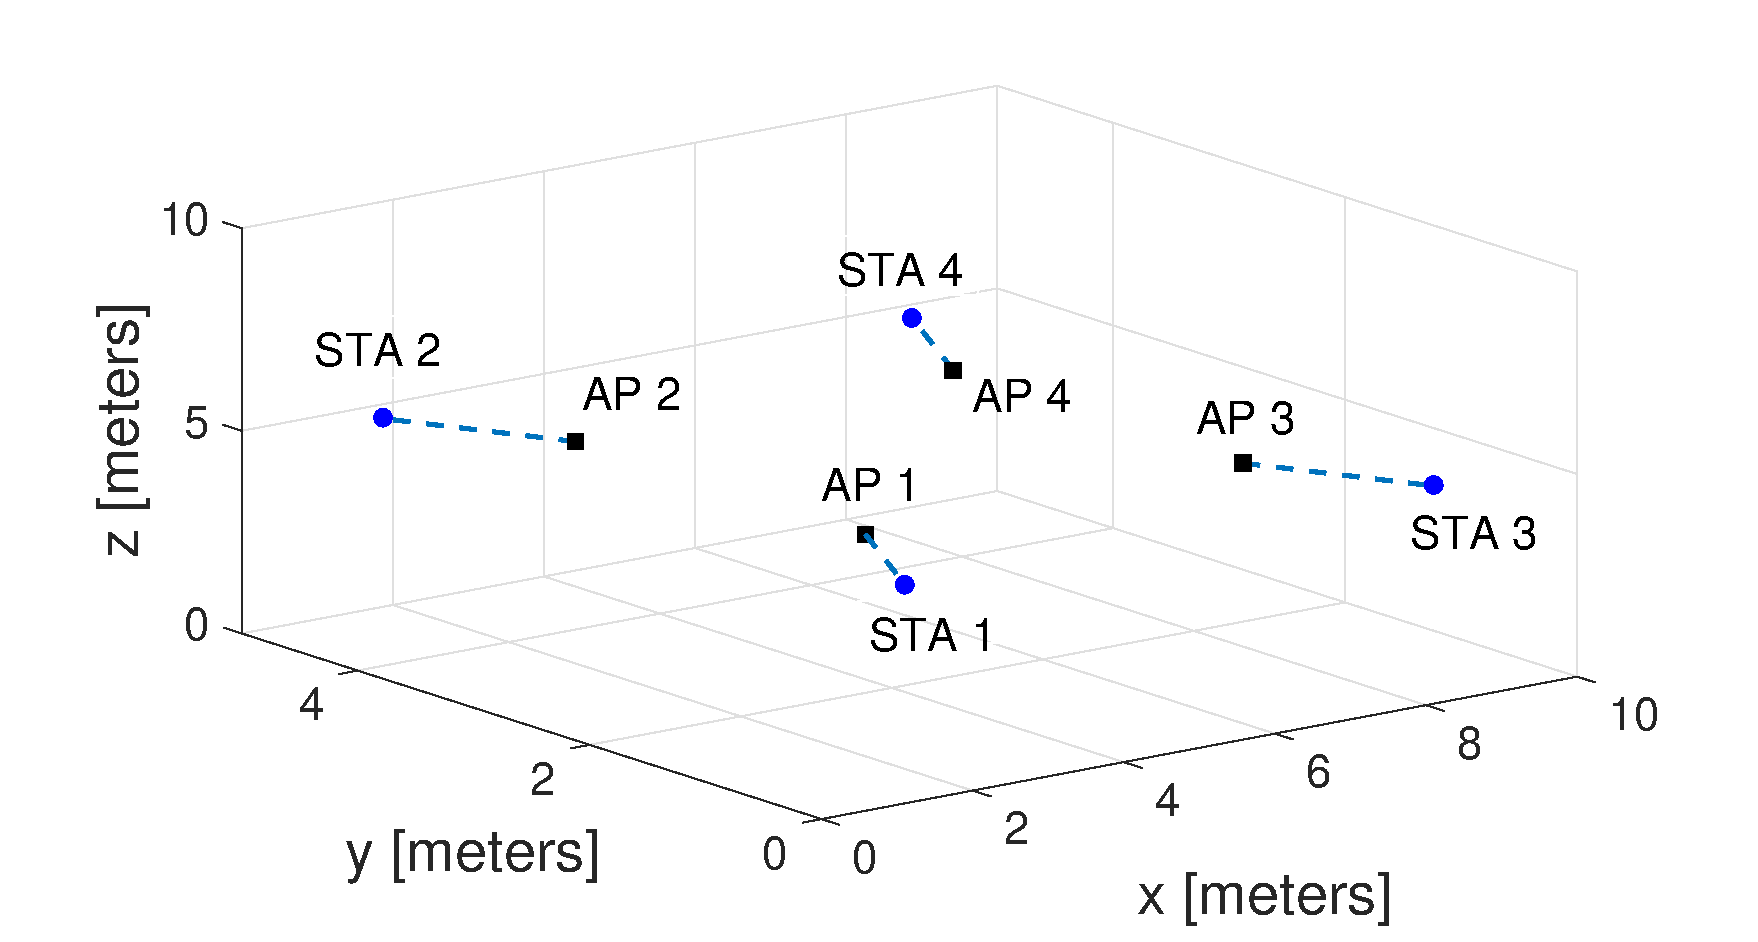
\includegraphics[width=\textwidth,height=0.32\textheight,keepaspectratio]{img/4_WLANs_scenario}
				\end{figure}
			\end{column}
		
		\end{columns}
	
	\end{block}	

	\begin{block}{Optimal solutions}
		\begin{itemize}
			\item \textbf{S1:} all WLANs must use $\text{CCA}_{max}$%\footnote{Optimal channel allocation is assumed}
			\item \textbf{S2:} all WLANs must use $\text{CCA}_{max}$ and $\text{Power}_{min}$
			\item \textbf{S3:} all WLANs must listen to the others 
		\end{itemize}
	\end{block}	

% Scenario
%	- different purposes
% 	- symmetric due to equal opportunities (in addition to aforementioned purposes)

\end{frame}

% Results: mean throughput per WLAN
\subsection{}
\begin{frame}{Selfish learning - Average throughput}

	%	
	\begin{columns}
		
		\begin{column}{4cm}
			\begin{figure}
				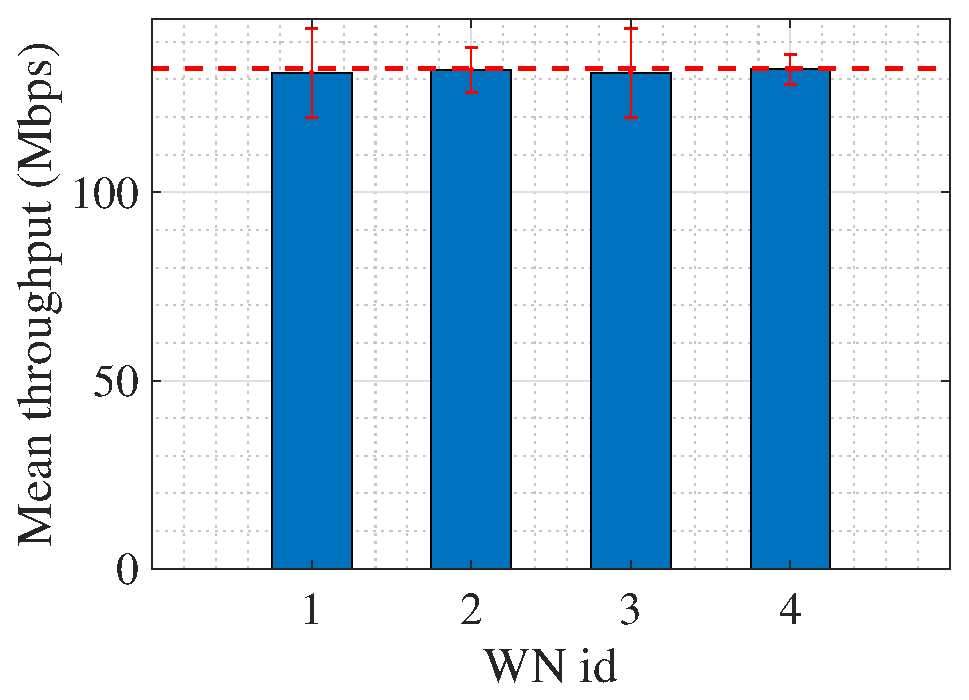
\includegraphics[width=\textwidth,height=0.4\textheight,keepaspectratio]{img/S1_ind_reward_mean_tpt_TS}
				\caption{S1}
			\end{figure}			
		\end{column}
		\hfill\vline\hfill
		\begin{column}{4cm}
			\begin{figure}
				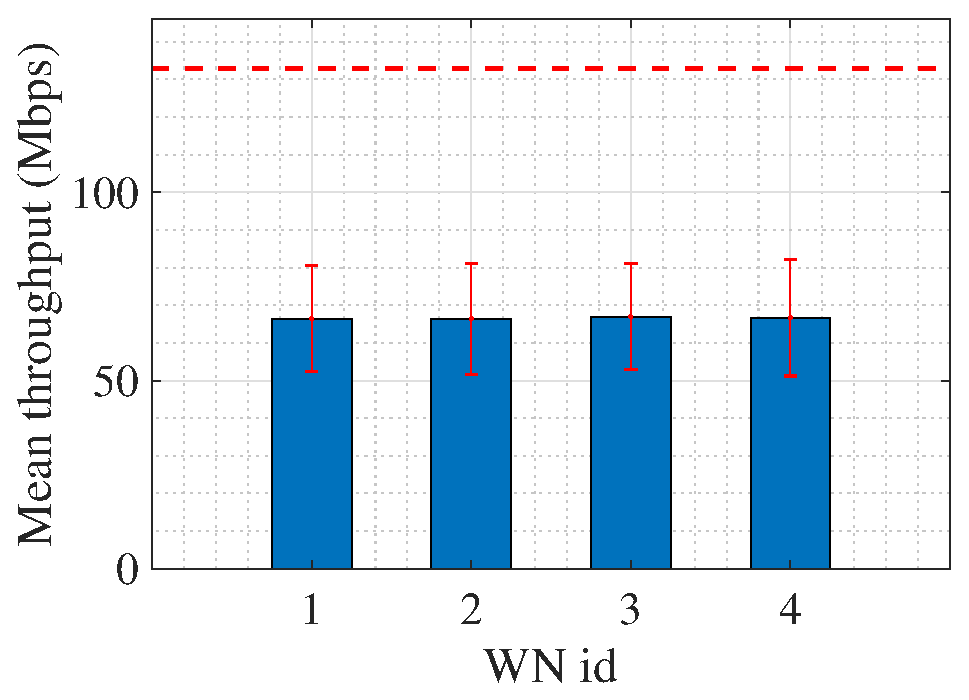
\includegraphics[width=\textwidth,height=0.4\textheight,keepaspectratio]{img/S2_ind_reward_mean_tpt_TS}
				\caption{S2}
			\end{figure}			
		\end{column}
		\hfill\vline\hfill
		\begin{column}{4cm}
			\begin{figure}
				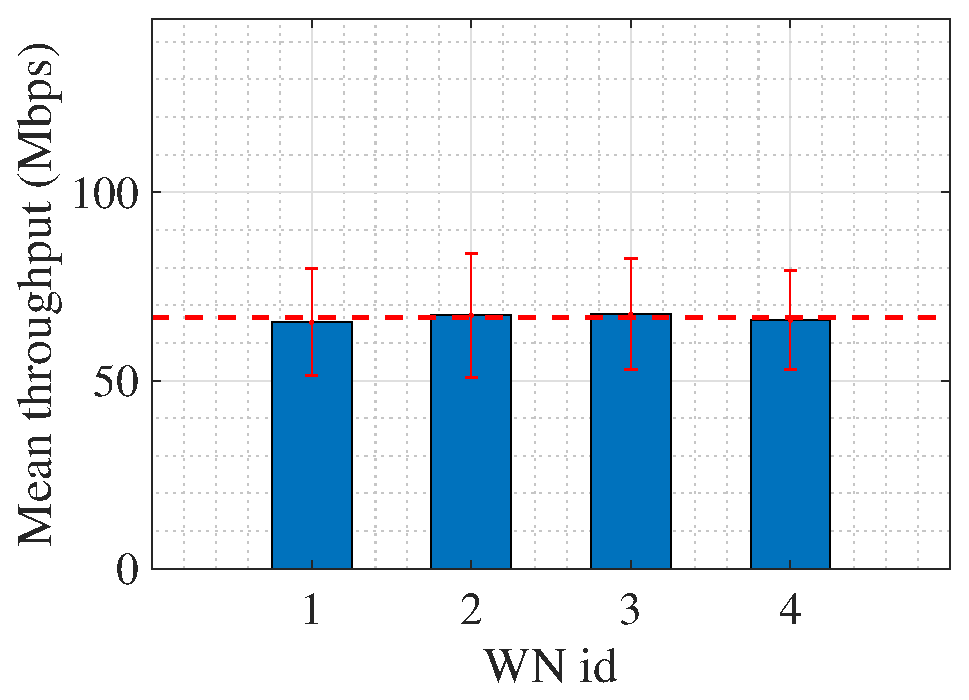
\includegraphics[width=\textwidth,height=0.4\textheight,keepaspectratio]{img/S3_ind_reward_mean_tpt_TS}
				\caption{S3}
			\end{figure}			
		\end{column}
		
	\end{columns}
	%\pause
	\begin{center}
		\begin{minipage}{15cm}			
			\begin{varblock}[9cm]{}
				\centering
				Convergence in terms of average throughput is reached in all the cases. However, it does not always match with the optimal solution.
			\end{varblock}
		\end{minipage}
	\end{center}	

\end{frame}

% Results - Individual throughput evolution
\subsection{}
\begin{frame}{Selfish learning - Individual throughput evolution}

%	
\begin{columns}
	
	\begin{column}{4cm}
		\begin{figure}
			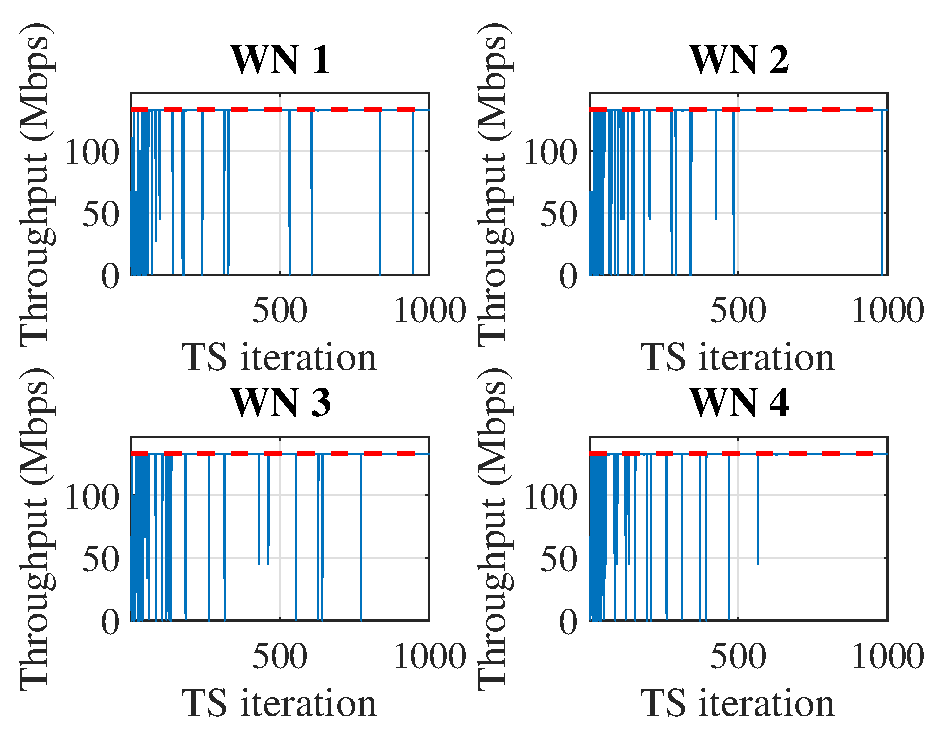
\includegraphics[width=\textwidth,height=0.4\textheight,keepaspectratio]{img/S1_ind_reward_temporal_individual_tpt_TS}
			\caption{S1}
		\end{figure}			
	\end{column}
	\hfill\vline\hfill
	\begin{column}{4cm}
		\begin{figure}
			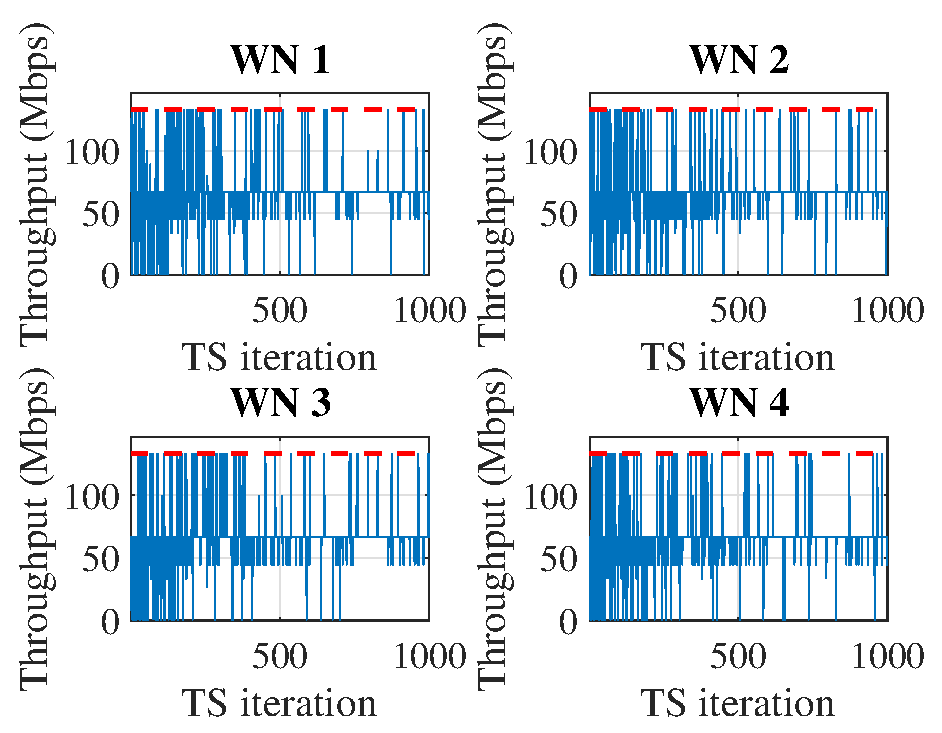
\includegraphics[width=\textwidth,height=0.4\textheight,keepaspectratio]{img/S2_ind_reward_temporal_individual_tpt_TS}
			\caption{S2}
		\end{figure}			
	\end{column}
	\hfill\vline\hfill
	\begin{column}{4cm}
		\begin{figure}
			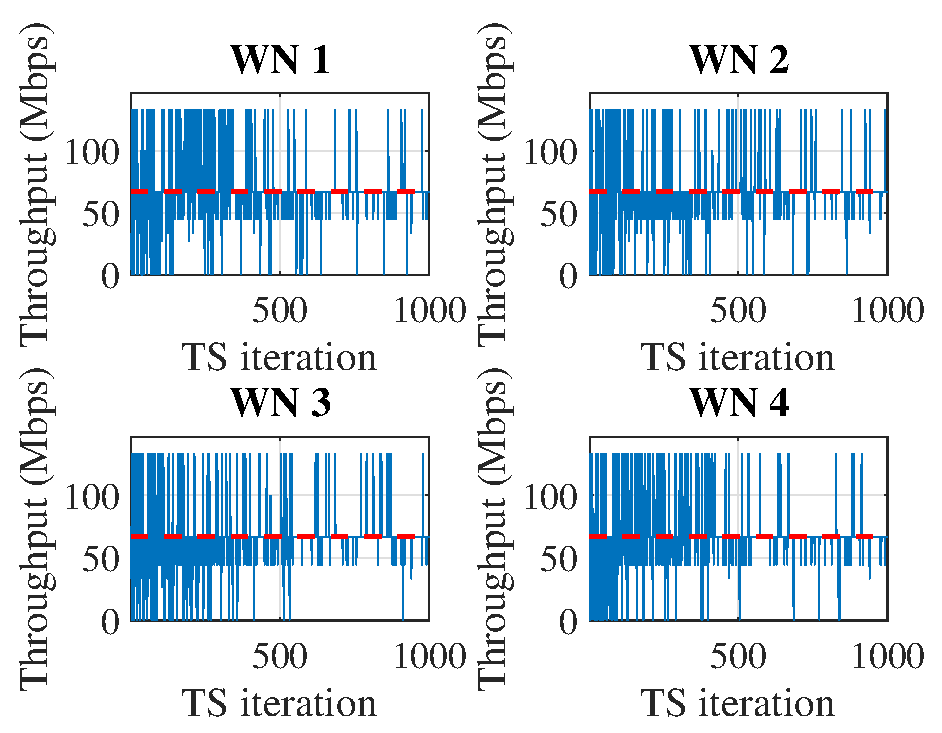
\includegraphics[width=\textwidth,height=0.4\textheight,keepaspectratio]{img/S3_ind_reward_temporal_individual_tpt_TS}
			\caption{S3}
		\end{figure}			
	\end{column}
	
\end{columns}
%\pause
\begin{center}
	\begin{minipage}{15cm}			
		\begin{varblock}[9cm]{}
			\centering
			A higher variability is observed in S2 and S3 (WLANs alternate good and bad performance). 
		\end{varblock}
	\end{minipage}
\end{center}	

\end{frame}

% Results - Actions probabilities
\subsection{}
\begin{frame}{Selfish learning - Actions probabilities}

%	
\begin{columns}
	
	\begin{column}{4cm}
		\begin{figure}
			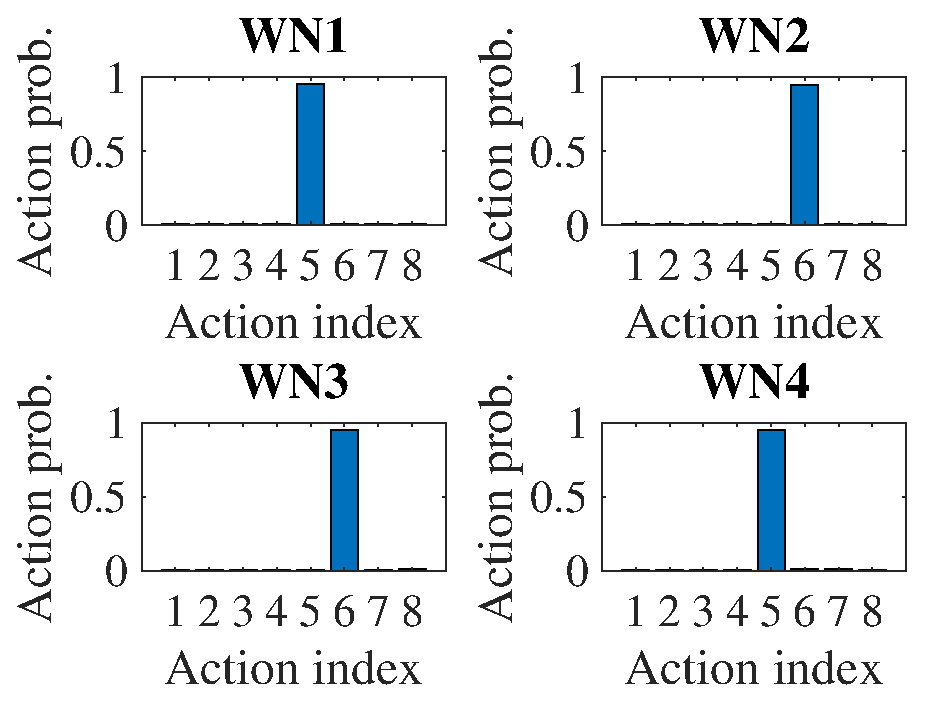
\includegraphics[width=\textwidth,height=0.4\textheight,keepaspectratio]{img/S1_ind_reward_actions_probability_TS}
			\caption{S1}
		\end{figure}			
	\end{column}
	\hfill\vline\hfill
	\begin{column}{4cm}
		\begin{figure}
			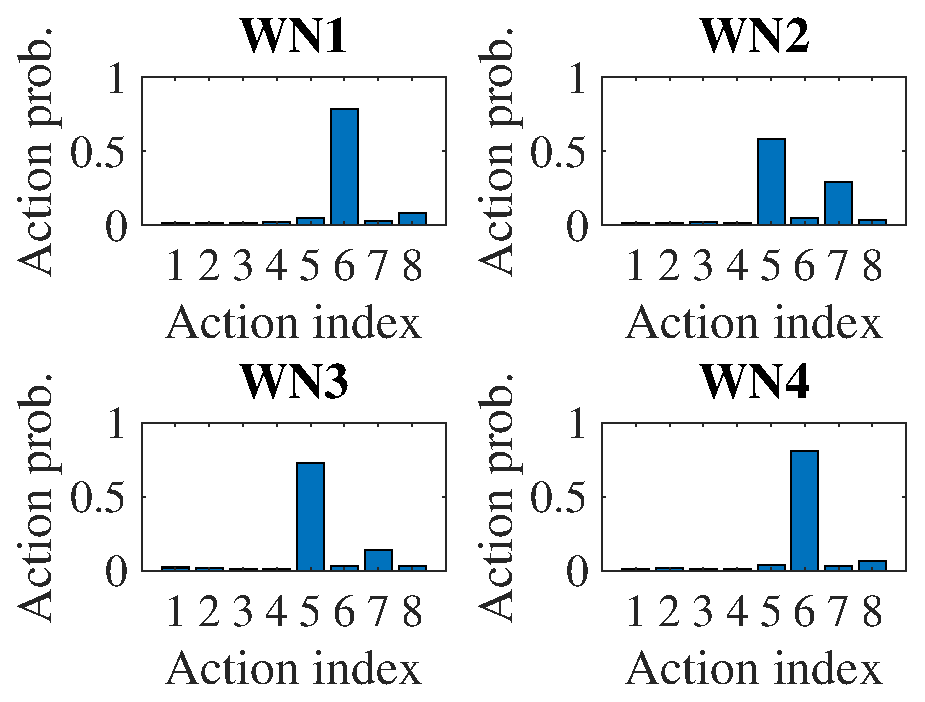
\includegraphics[width=\textwidth,height=0.4\textheight,keepaspectratio]{img/S2_ind_reward_actions_probability_TS}
			\caption{S2}
		\end{figure}			
	\end{column}
	\hfill\vline\hfill
	\begin{column}{4cm}
		\begin{figure}
			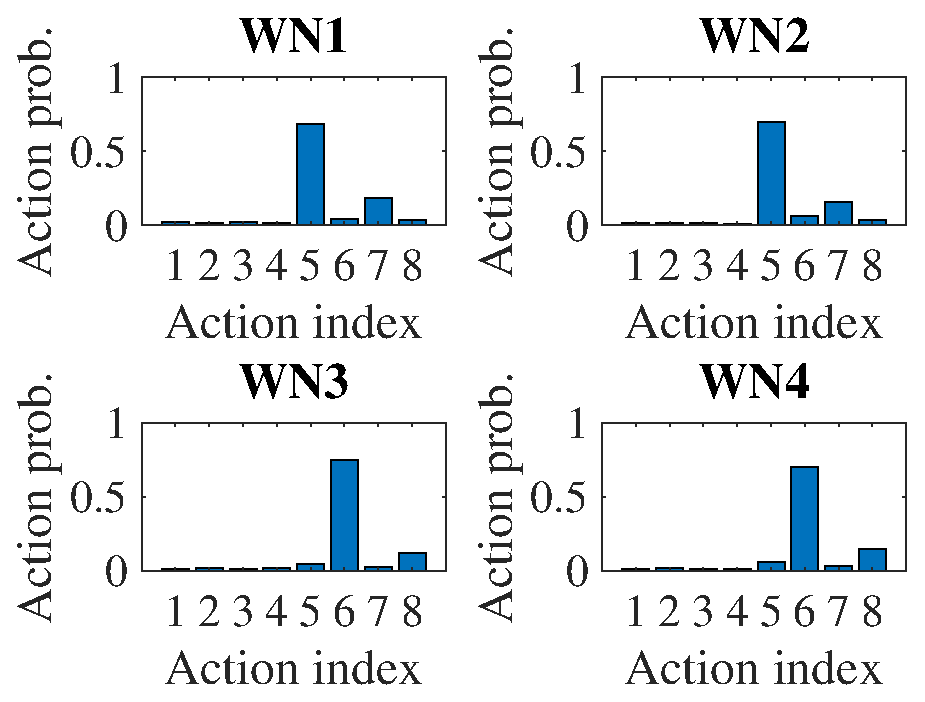
\includegraphics[width=\textwidth,height=0.4\textheight,keepaspectratio]{img/S3_ind_reward_actions_probability_TS}
			\caption{S3}
		\end{figure}			
	\end{column}
	
\end{columns}
%\pause
\begin{center}
	\begin{minipage}{15cm}			
		\begin{varblock}[9cm]{}
			\centering
			WLANs in S1 rapidly achieve a single preferred action, while in S2 and S3 they use more actions.
		\end{varblock}
	\end{minipage}
\end{center}	

\end{frame}

% Impact on leagy nodes
\subsection{}
\begin{frame}{Impact on legacy networks - Scenario}

	\begin{columns}
		
		\begin{column}{6.5cm}
			\begin{block}{Random scenario}
				\begin{itemize}
					\item We test different \% of legacy networks (randomly chosen)
					\item Goal: to study the performance of both learning and legacy networks
				\end{itemize}
			\end{block}	
		\end{column}
		%\pause
		\begin{column}{5cm}
			\begin{figure}
				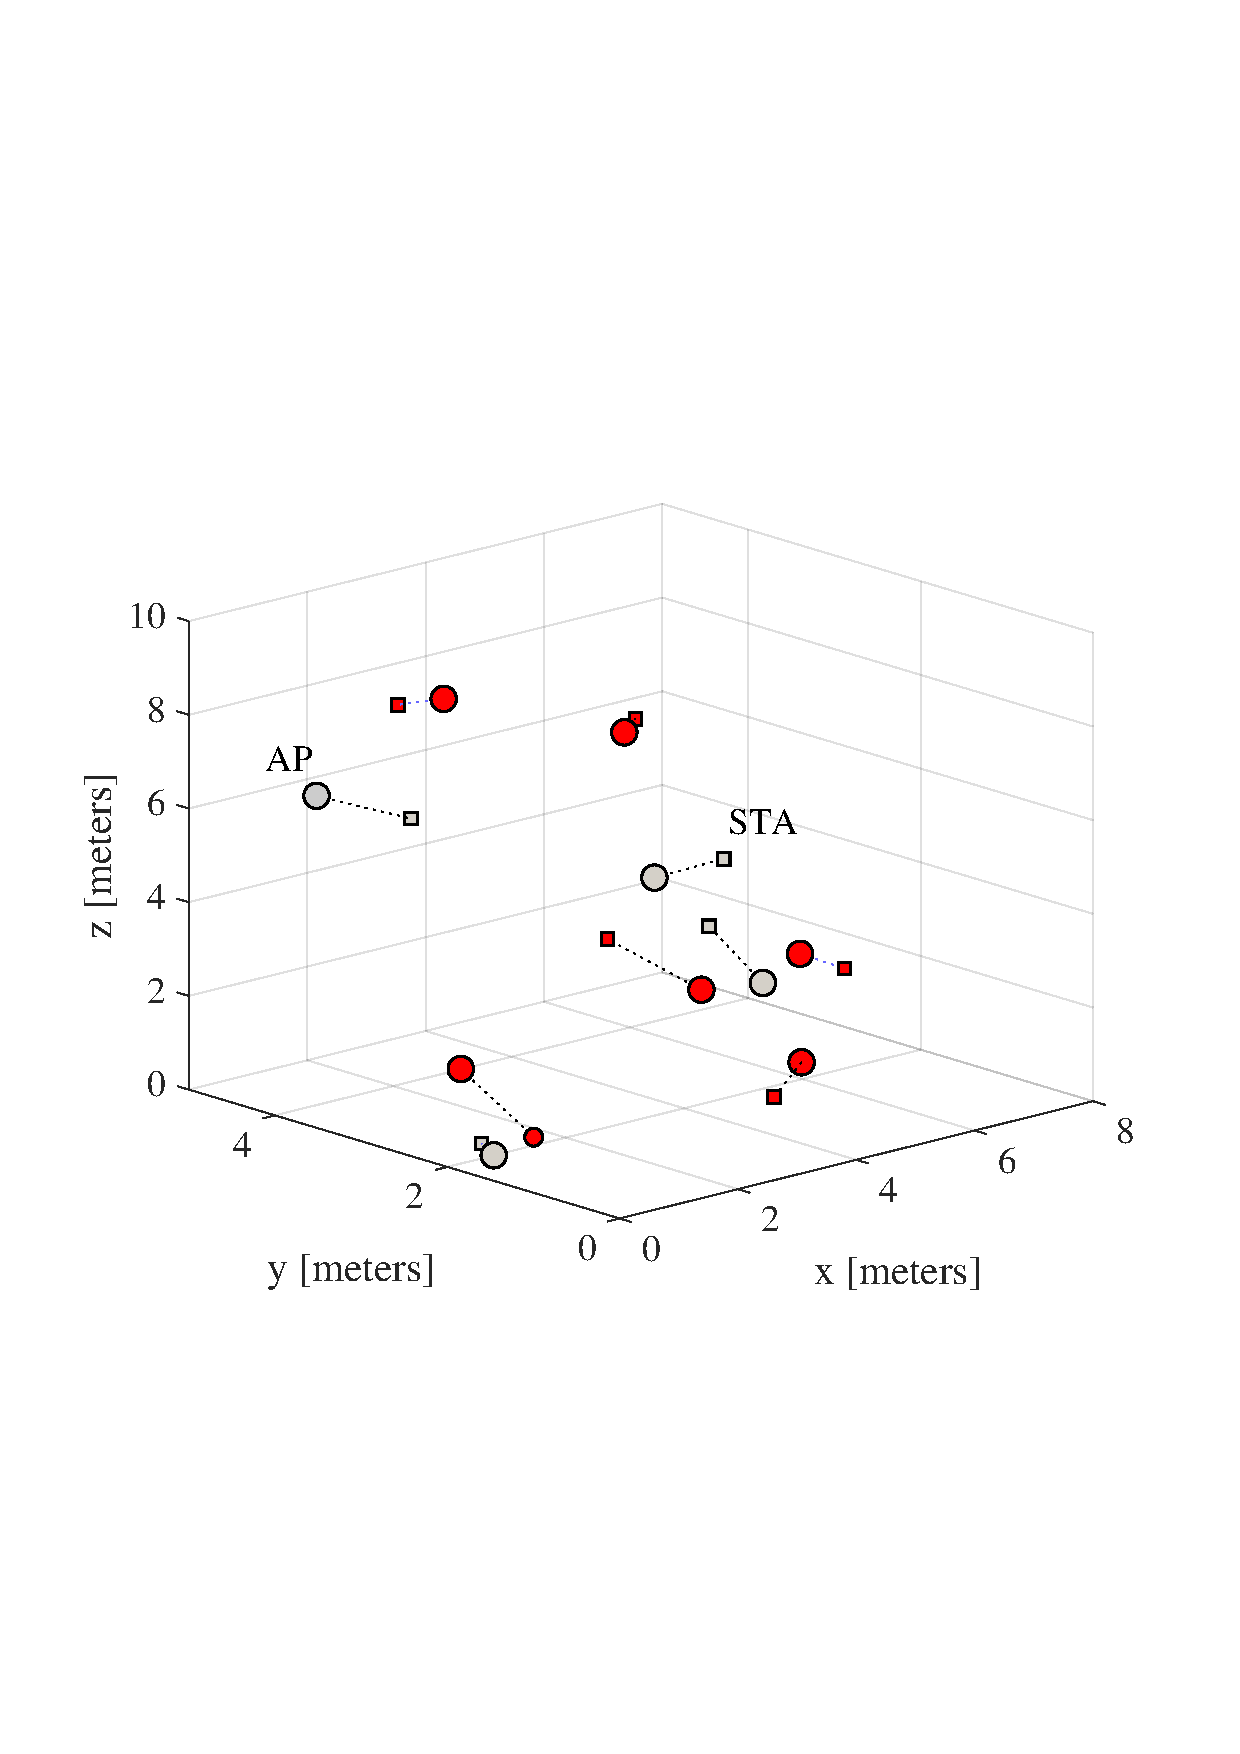
\includegraphics[width=\textwidth,height=1\textheight,keepaspectratio]{img/random_scenario}
			\end{figure}
		\end{column}	
	
	\end{columns}

\end{frame}

% Impact on leagy nodes
\subsection{}
\begin{frame}{Impact on legacy networks - Results}

	\begin{figure}[h!]
		\centering
		\begin{subfigure}[b]{0.3\textwidth}
			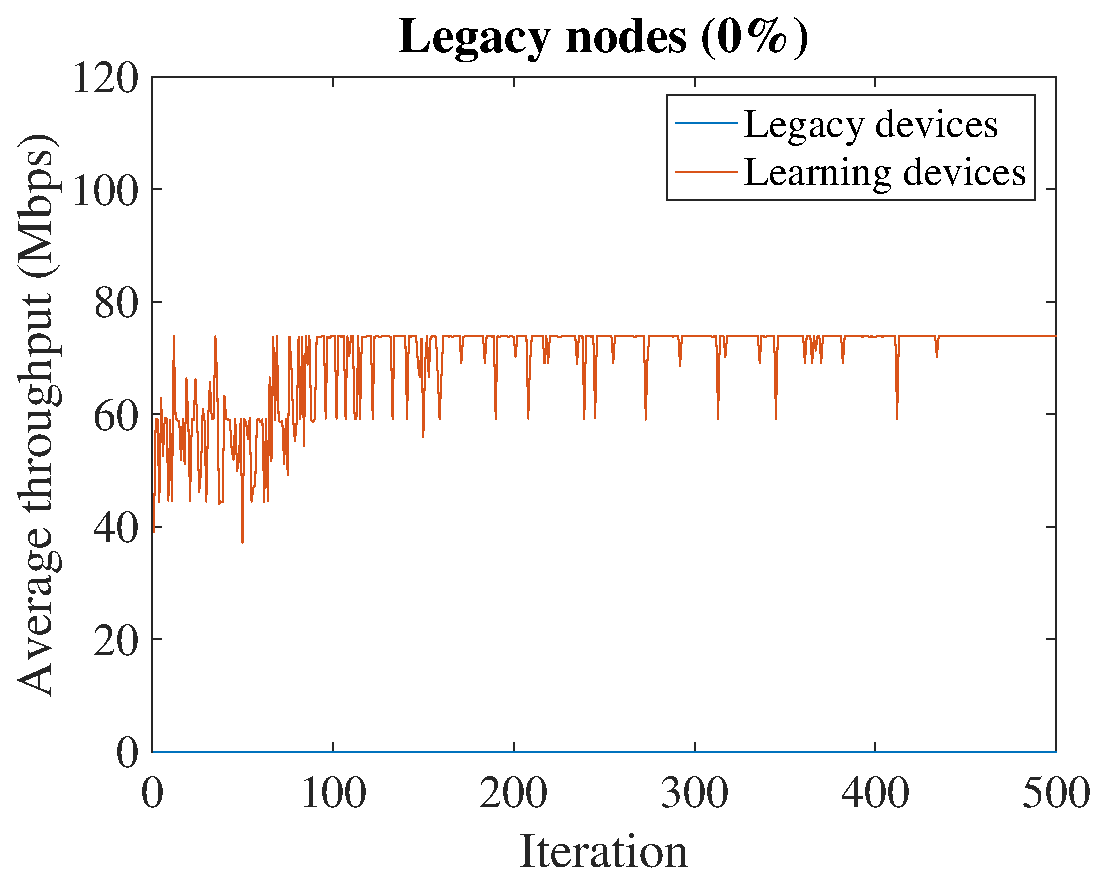
\includegraphics[width=\textwidth]{img/learning_vs_legacy_0_legacy__500_iterations}
			\caption{0/8 legacy (0\%)}
		\end{subfigure}
		\begin{subfigure}[b]{0.3\textwidth}
			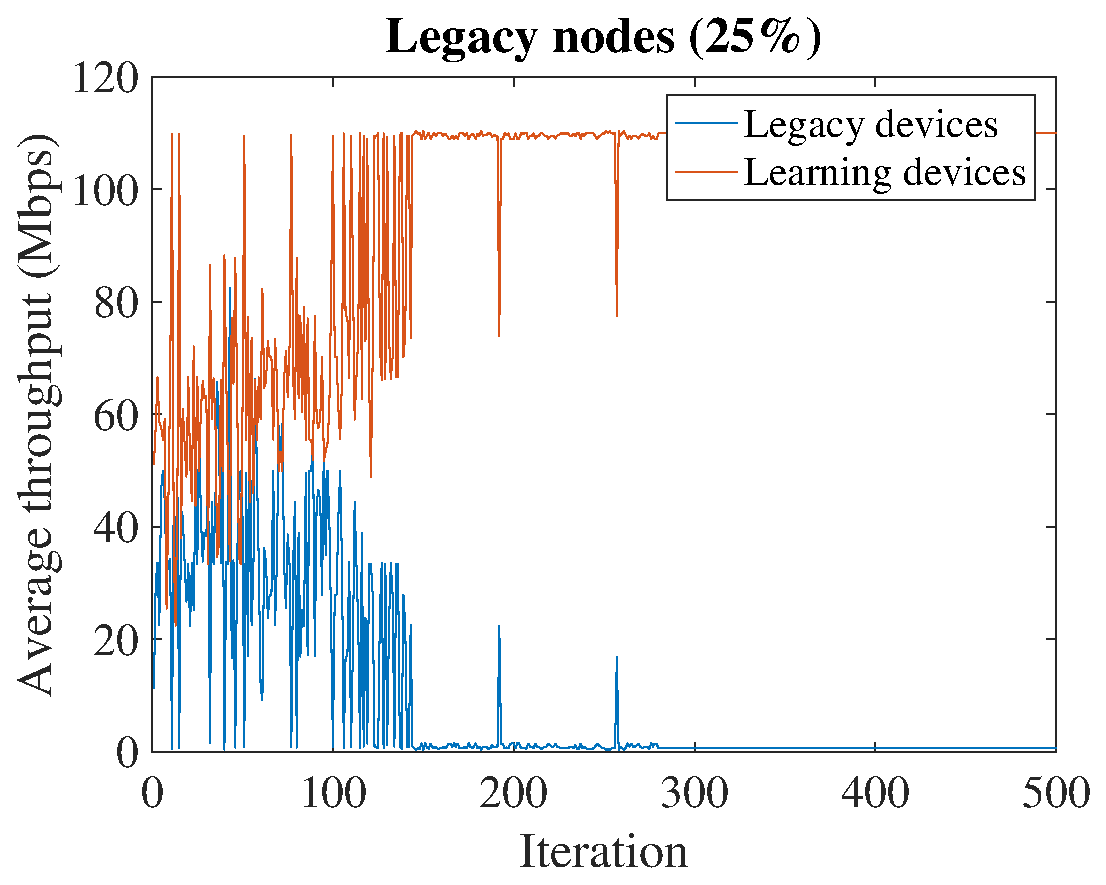
\includegraphics[width=\textwidth]{img/learning_vs_legacy_25_legacy__500_iterations}
			\caption{2/8 legacy (25\%)}
		\end{subfigure}
		\\
		\begin{subfigure}[b]{0.3\textwidth}
			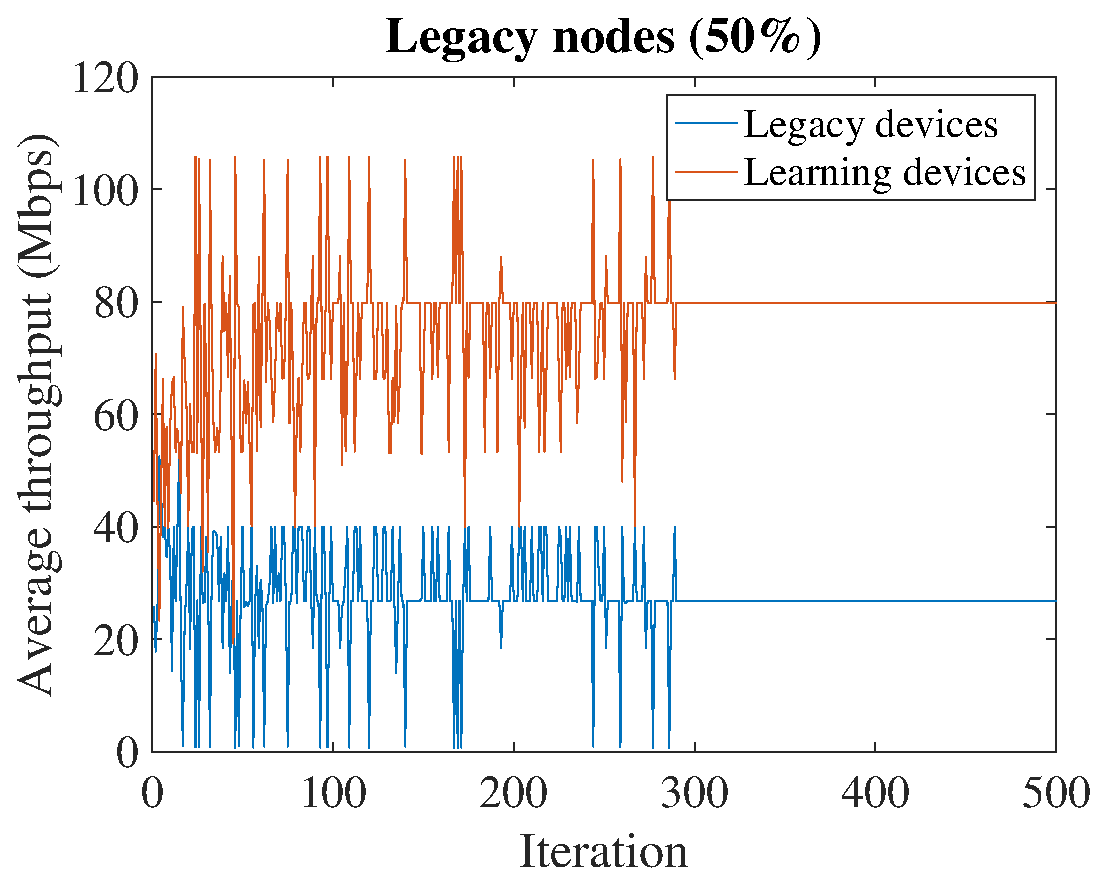
\includegraphics[width=\textwidth]{img/learning_vs_legacy_50_legacy__500_iterations}
			\caption{4/8 legacy (50\%)}
		\end{subfigure}
		\begin{subfigure}[b]{0.3\textwidth}
			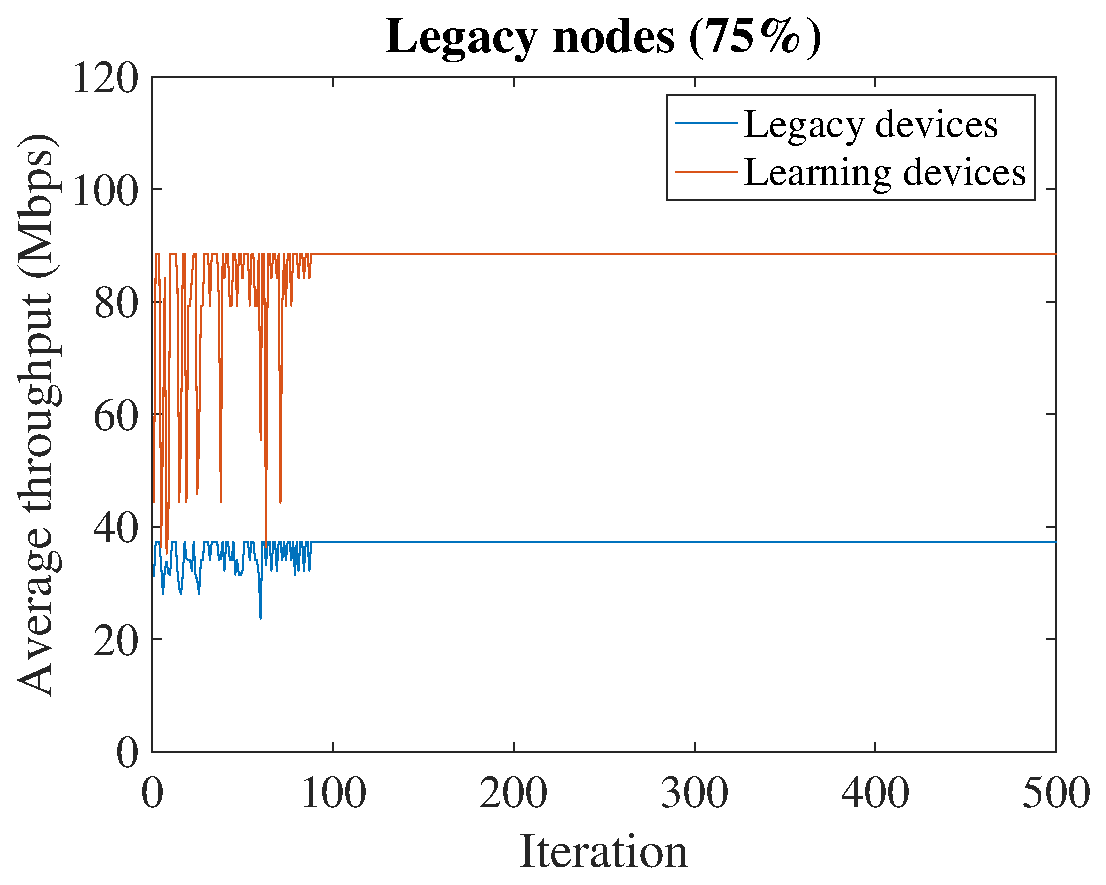
\includegraphics[width=\textwidth]{img/learning_vs_legacy_75_legacy__500_iterations}
			\caption{6/8 legacy (75\%)}
		\end{subfigure}
	\end{figure}

\end{frame}

%%% CONCLUSIONS
\section{Conclusions}

%\subsection{}
%\begin{frame}{Summary}
%
%	\begin{itemize}
%		%\item Reinforcement Learning is key for dealing with uncertainty	in decentralized wireless networks
%		\item The application of MABs for the SR problem was studied 
%		\item A realistic simulation was provided to study the effects of learning in Wireless Networks
%		\item It was shown that equilibriums can be achieved, even if the optimal solution cannot obtained
%		\item It was shown that learning selfishly may harm the performance of static networks
%		%\item The learning time must be taken into account
%%		\item In order to gain efficiency, It is important to exploit the characteristics of each problem
%%		\begin{itemize}
%%			\item Stochastic vs Non-stochastic bandits
%%			\item Contextual, Combinatorial bandits
%%		\end{itemize}	
%	\end{itemize}	
%
%\end{frame}

\subsection{}
\begin{frame}{Decentralized learning}

	%\pause

	\begin{alertblock}{Challenges}
		\begin{itemize}
			\item Finding equilibriums
			\item Fairness and asymmetries in a network			
		\end{itemize}
	\end{alertblock}	

	%\pause
	
	\begin{exampleblock}{Opportunities}
		\begin{itemize}
			\item Behavior inference (work in progress)
			\item Usage of constraints to favor fairness
			\item Exploitation of problem's characteristics for fast convergence (contextual, combinatorial bandits)
		\end{itemize}
	\end{exampleblock}	
	
\end{frame}

\subsection{}
\begin{frame}{Centralized and Collaborative learning}

	%\pause

	\begin{alertblock}{Challenges}
		\begin{itemize}
			\item Increased complexity
			\item Communication overheads (is it worth?)
		\end{itemize}
	\end{alertblock}	

	%\pause
	
	\begin{exampleblock}{Opportunities}
		\begin{itemize}
			\item More control
			\item Less variability
			\item Correlated equilibria
		\end{itemize}
	\end{exampleblock}	

\end{frame}

\section{}
\begin{frame}{Any questions?}
\begin{figure}
	
\includegraphics[width=\textwidth,height=0.4\textheight,keepaspectratio]{img/question_mark.png}
\end{figure}

\begin{center}
	
	\footnotesize
	\textbf{Francesc Wilhelmi}\\
	\textcolor{blue}{francisco.wilhelmi@upf.edu}\\
	PhD student\\
	Department of Communication and Information Technologies\\
	Universitat Pompeu Fabra (Barcelona)
\end{center}

\end{frame}

\appendix
\backupbegin

% Backup slides here

% RL
\subsection{}
\begin{frame}{Backup: Reinforcement Learning}

\begin{columns}
	\begin{column}{6.5cm}
		\begin{block}{Goal}
			An agent attempts to learn a policy given the observations it does. The goal is to maximize the expected future cumulative reward.
			\begin{itemize} 
				\item No supervisor (only reward signal)
				\item Delayed feedback \& sequentiality
				\item Actions affect the environment
			\end{itemize}
		\end{block}
	\end{column}
\begin{column}{5cm}	
		\begin{figure}
			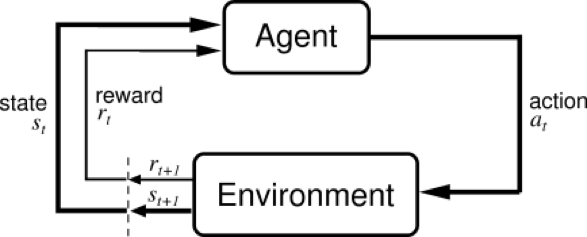
\includegraphics[width=\textwidth,height=0.4\textheight,keepaspectratio]{img/rl}
		\end{figure}
		$\mathcal{M} = \{\mathcal{S, A, R, T}\}$
		\begin{itemize}
			\item $\mathcal{S}$: set of states
			\item $\mathcal{A}$: set of actions
			\item $\mathcal{R}$: set of rewards
			\item $\mathcal{T}$: transitions probabilities
		\end{itemize}
	\end{column}	
\end{columns}
\end{frame}

% MABs overview
\subsection{}
\begin{frame}{Backup: Multi-Armed Bandits}
	\begin{columns}
		\begin{column}{6.5cm}
			Frames the exploration/exploitation trade-off. The hidden reward distributions must be learned while maximizing the gains. 
			\begin{itemize}
				\item Action-selection strategies to cope with hidden distributions ($\varepsilon$-greedy, EXP3, UCB…)
				\item Several variants (contextual, adversarial, stochastic, restless…)
				\item States-independent
				\item Reward becomes regret: $R_n = \sum_{t=1}^{n} l_{t,I_t} - \text{min}_{i \in K} \sum_{t=1}^{n} l_{t,i}$
			\end{itemize}
		\end{column}
		\begin{column}{5cm}	
			\begin{figure}
				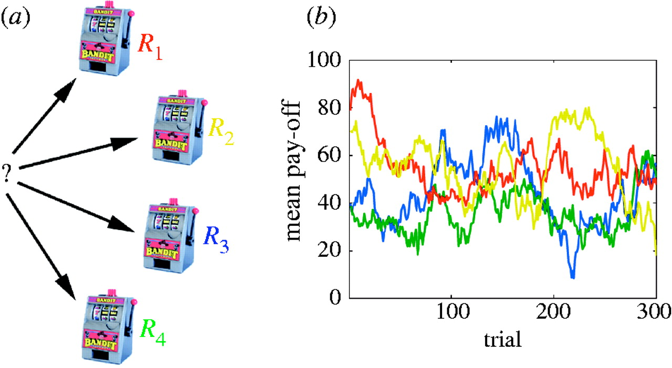
\includegraphics[width=\textwidth,height=0.4\textheight,keepaspectratio]{img/hidden_reward}
			\end{figure}	
		\end{column}	
	\end{columns}	
\end{frame}

% Thompson sampling
\subsection{}
\begin{frame}{Backup: Thompson sampling}
	% Action-selection strategy
	%	- TS explanation
	% 	- Algorithm 
	Thompson sampling [19] is a Bayesian action-selection technique 
	\begin{itemize}
		\item It constructs a probabilistic model of the rewards and assumes a prior distribution of the parameters of said model
		\item Keeps track of the posterior distribution of the rewards, and pulls arms randomly in a way that the drawing probability of each arm matches the probability of the particular arm being optimal
		%Given the data collected during the learning procedure, this policy keeps track of the posterior distribution of the rewards, and pulls arms randomly in a way that the drawing probability of each arm matches the probability of the particular arm being optimal. In practice, this is implemented by sampling the parameter corresponding to each arm from the posterior distribution, and pulling the arm yielding the maximal expected reward under the sampled parameter value.
		\item For the sake of practicality, we aim to apply Thompson sampling using a Gaussian model for the rewards with a standard Gaussian prior as suggested in [20].
		\item In adversarial wireless networks, it has been shown to perform better than using the magnitude of the reward [9]
	\end{itemize}
	% By standard calculations, it can be verified that the posterior distribution of the rewards under this model is Gaussian with mean 
	%\begin{equation}
	%\hat{r}_k(t) = \frac{\sum_{w=1:k}^{t-1} r_k(t) }{n_k(t) + 1}
	%\nonumber
	%\end{equation}
	%and variance $\sigma_k^2(t) = \frac{1}{n_k + 1}$, where $n_k$ is the number of times that arm $k$ was drawn until the beginning of round $t$. Thus, implementing Thompson sampling in this model amounts to sampling a parameter $\theta_k$ from the Gaussian distribution $\mathcal{N}\left(\hat{r}_k(t),\sigma_k^2(t)\right)$ and choosing the action with the maximal parameter. 
\end{frame}

% Thompson sampling - Algorithm
\subsection{}
\begin{frame}{Backup: Applied Thompson sampling}
	\begin{figure}
		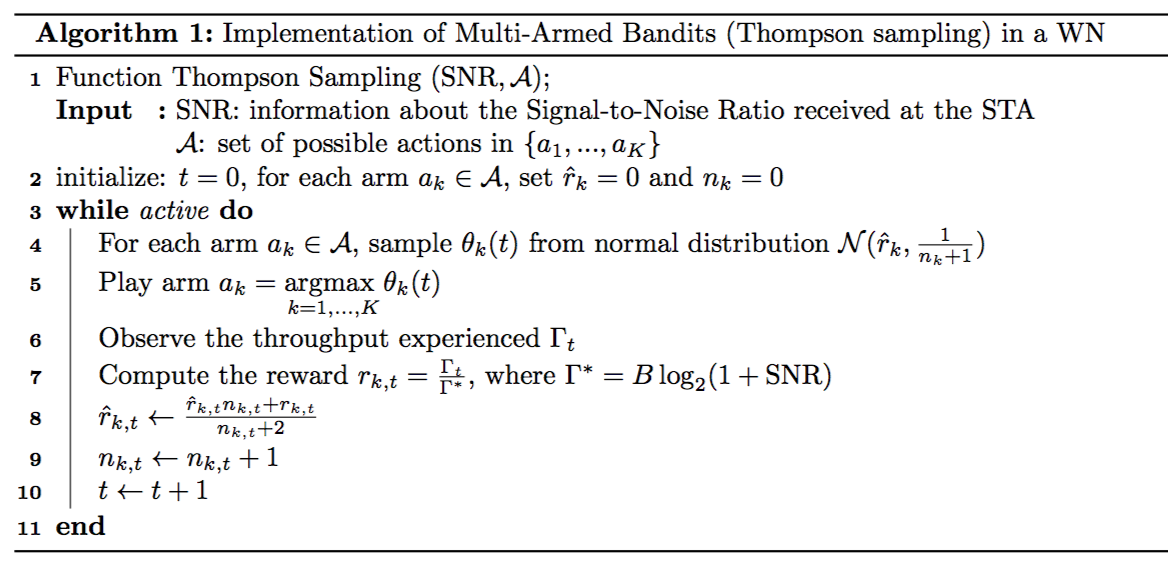
\includegraphics[width=\textwidth,height=0.65\textheight,keepaspectratio]{img/thompson_sampling}
	\end{figure}
\end{frame}

\backupend

% References 
\begin{frame}{References}
\tiny
\begin{itemize}
	
	\citem{1} Afaqui, M. Shahwaiz, et al. "Evaluation of dynamic sensitivity control algorithm for IEEE 802.11 ax." Wireless Communications and Networking Conference (WCNC), 2015 IEEE. IEEE, 2015.
	
	\citem{2} KLAINE, Paulo Valente, et al. A Survey of Machine Learning Techniques Applied to Self-Organizing Cellular Networks. IEEE Communications Surveys \& Tutorials, 2017, vol. 19, no 4, p. 2392-2431.	
	
	\citem{3} BKASSINY, Mario; LI, Yang; JAYAWEERA, Sudharman K. A survey on machine-learning techniques in cognitive radios. IEEE Communications Surveys \& Tutorials, 2013, vol. 15, no 3, p. 1136-1159.
	
	\citem{4} ALSHEIKH, Mohammad Abu, et al. Machine learning in wireless sensor networks: Algorithms, strategies, and applications. IEEE Communications Surveys \& Tutorials, 2014, vol. 16, no 4, p. 1996-2018.
	
	\citem{5} DI, Ma; JOO, Er Meng. A survey of machine learning in wireless sensor netoworks from networking and application perspectives. En Information, Communications \& Signal Processing, 2007 6th International Conference on. IEEE, 2007. p. 1-5.
	
	\citem{6} FORSTER, Anna. Machine learning techniques applied to wireless ad-hoc networks: Guide and survey. En Intelligent Sensors, Sensor Networks and Information, 2007. ISSNIP 2007. 3rd International Conference on. IEEE, 2007. p. 365-370.
	
	\citem{7} Nie, J., \& Haykin, S. (1999). A Q-learning-based dynamic channel assignment technique for mobile communication systems. IEEE Transactions on Vehicular Technology, 48(5), 1676-1687.
	
	\citem{8} Li, H. (2009, October). Multi-agent Q-learning of channel selection in multi-user cognitive radio systems: A two by two case. In Systems, Man and Cybernetics, 2009. SMC 2009. IEEE International Conference on (pp. 1893-1898). IEEE.
	
	\citem{9} Sallent, O., Pérez-Romero, J., Ferrús, R., \& Agustí, R. (2015, June). Learning-based coexistence for LTE operation in unlicensed bands. In Communication Workshop (ICCW), 2015 IEEE International Conference on (pp. 2307-2313). IEEE.
	
	\citem{10} Rupasinghe, N., \& Güvenç, İ. (2015, March). Reinforcement learning for licensed-assisted access of LTE in the unlicensed spectrum. In Wireless Communications and Networking Conference (WCNC), 2015 IEEE (pp. 1279-1284). IEEE. 
	
\end{itemize}

\end{frame}

\begin{frame}{References}
\tiny
\begin{itemize}	
	
	\citem{11} Bennis, M., \& Niyato, D. (2010, December). A Q-learning based approach to interference avoidance in self-organized femtocell networks. In GLOBECOM Workshops (GC Wkshps), 2010 IEEE (pp. 706-710). IEEE.
	
	\citem{12} Bennis, M., Guruacharya, S., \& Niyato, D. (2011, December). Distributed learning strategies for interference mitigation in femtocell networks. In Global Telecommunications Conference (GLOBECOM 2011), 2011 IEEE (pp. 1-5). IEEE.
	
	\citem{13} Maghsudi, S., \& Stańczak, S. (2015). Joint channel selection and power control in infrastructureless wireless networks: A multiplayer multiarmed bandit framework. IEEE Transactions on Vehicular Technology, 64(10), 4565-4578. 
	
	\citem{14} Maghsudi, S., \& Stańczak, S. (2015). Channel selection for network-assisted D2D communication via no-regret bandit learning with calibrated forecasting. IEEE Transactions on Wireless Communications, 14(3), 1309-1322.
	
	\citem{15} Wilhelmi, F., Cano, C., Neu, G., Bellalta, B., Jonsson, A., \& Barrachina-Muñoz, S. (2017). Collaborative Spatial Reuse in Wireless Networks via Selfish Multi-Armed Bandits. arXiv preprint arXiv:1710.11403.
		
	\citem{16} Gai, Y., Krishnamachari, B., \& Jain, R. (2012). Combinatorial network optimization with unknown variables: Multi-armed bandits with linear rewards and individual observations. IEEE/ACM Transactions on Networking (TON), 20(5), 1466-1478.
	
	\citem{17} Combes, R., \& Proutiere, A. (2015). Dynamic rate and channel selection in cognitive radio systems. IEEE Journal on Selected Areas in Communications, 33(5), 910-921. 
	
\end{itemize}

\end{frame}

\begin{frame}{References}
\tiny
\begin{itemize}

\citem{18} Liu, K., \& Zhao, Q. (2010). Distributed learning in multi-armed bandit with multiple players. IEEE Transactions on Signal Processing, 58(11), 5667-5681.

\citem{19} Thompson, W. R. (1933). On the likelihood that one unknown probability exceeds another in view of the evidence of two samples. Biometrika, 25, 285-294.

\citem{20} Agrawal, S., \& Goyal, N. (2013, April). Further optimal regret bounds for thompson sampling. In Artificial Intelligence and Statistics (pp. 99-107).

\end{itemize}

\end{frame}

\end{document}